\section{Fuzzy rules}

\begin{definition}
    A \emph{fuzzy rule} is a rule whose clauses have the form "V is L", where V is a linguistic variable, and L is a label representing a value for V associated with a fuzzy set.
    Each of these clauses is referred to as a \emph{linguistic clause}. 
\end{definition}
Often, clauses in the antecedent are implicitly connected by the AND operator, which is not explicitly written.
The antecedent is typically compared to facts represented as values of base variables corresponding to the linguistic variables. 
The consequent can be one of two types:
\begin{itemize}
    \item Linguistic rules: the consequent is a conjunction of linguistic clauses. 
        These rules can be viewed as a mapping between the interpretation of an input configuration and a symbolic description of the desired output. 
        The general formula is:
        \[\textnormal{IF }(\textnormal{A is }L_{A_i})\textnormal{ AND }(\textnormal{B is }L_{B_k})\textnormal{ AND }\dots\textnormal{ THEN }(\textnormal{U is }L_{U_m})\textnormal{ AND }\dots\]
    \item Model rules: associate a model with the linguistic interpretation of its applicability conditions. 
        This can be seen as a mapping between the interpretation of an input configuration and a model that is applied to the input real values to obtain the output. 
        The general formula is:
        \[\textnormal{IF }(\textnormal{A is }L_{A_n})\textnormal{ AND }(\textnormal{B is }L_{B_k})\textnormal{ AND }\dots\textnormal{ THEN } \textnormal{U is } f(\textnormal{A,B})\]
\end{itemize}
The steps for using fuzzy rules are as follows:
\begin{enumerate}
    \item Input matching.
    \item Combining matching degrees.
    \item Combining with rule weight, if present.
    \item Aggregating output from different rules.
    \item Optionally, defuzzification of the output.
\end{enumerate}

When defuzzifying the output, various operators can be considered in addition to the weighted mean. 
These operators include the centroid, bisector, average of maxima, the lowest maximum, the highest maximum, center of the highest area, and more. 
The choice of operator can impact the system's output and the level of optimization.
\begin{example}
    Let's consider the following scenario:
    \begin{itemize}
        \item Two input variables, A and B, each with fuzzy partitions distributed equally from Negative Large to Positive Large.
        \item One output variable U (equally distributed fuzzy set) from Negative Large to Positive Large. The fuzzy sets are all singletons.
    \end{itemize} 
    \begin{figure}[H]
        \centering
        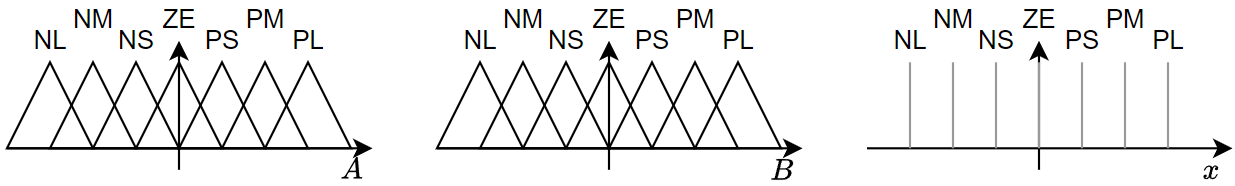
\includegraphics[width=0.5\linewidth]{images/rules.png}
    \end{figure}
    To define the rules of the rule base, along with their weights, we have the following rules:
    \begin{enumerate}
        \item IF A is $PL$ AND B is $PS$ THEN X is $PM$ (weight 1).
        \item IF A is $PM$ AND B is $PS$ THEN X is $PS$ (weight 0.5).
        \item IF A is $PL$ AND B is $PM$ THEN X is $PM$ (weight 1).
    \end{enumerate}
    Now, let's set A to 22 and B to 140. 
    The steps used to calculate the output value are as follows:
    \begin{enumerate}
        \item For the first step, we need to check the corresponding truth value for each label:
            \begin{itemize}
                \item (A is $PL$) has a truth value of 0.2.
                \item (B is $PS$) has a truth value of 0.6.
                \item (A is $PM$) has a truth value of 0.8.
                \item (B is $PM$) has a truth value of 0.4.
            \end{itemize}
        \item To consider the degree of truth of each predicate, we simply take the minimum between the two values (due to the AND operator). 
            Thus, we get: 
            \begin{itemize}
                \item 0.2 for the first rule. 
                \item 0.6 for the second. 
                \item 0.4 for the third.
            \end{itemize}
        \item Now we have to consider the rule weight. 
            To do this, we select the minimum between the previously calculated value and the weight value. 
            So, the final values for the consequents are as follows:
            \begin{itemize}
                \item 0.2 for the first rule. 
                \item 0.5 for the second. 
                \item 0.4 for the third.
            \end{itemize}
        \item To aggregate the output, we take the maximum value when we have a repeated expression. 
            In this case, we obtain that: 
            \begin{itemize}
                \item (X is $PM$) has a truth value of 0.4.
                \item (X is $PS$) has a truth value of 0.5.
            \end{itemize}
            This result can be visualized graphically by cutting the initial graph: 
            \begin{figure}[H]
                \centering
                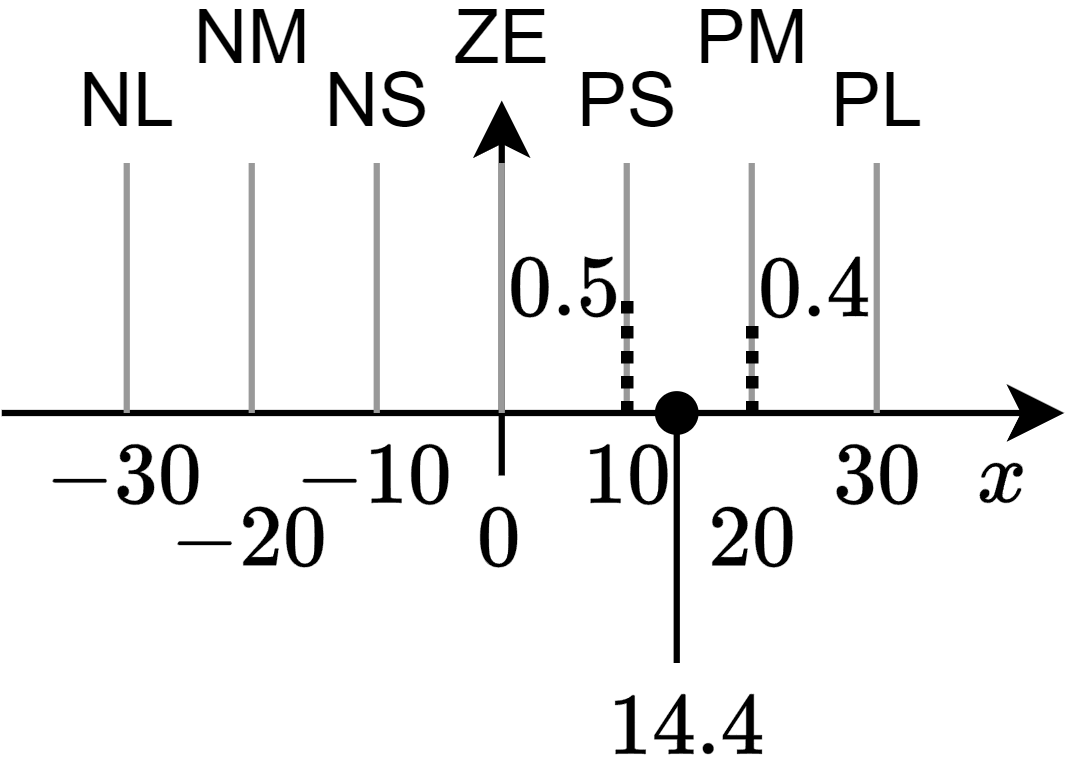
\includegraphics[width=0.4\linewidth]{images/cut.png}
            \end{figure}
        \item Finally, to defuzzify the result and obtain a numerical value, we can use a simple weighted mean:
            \[\textnormal{U}=\dfrac{10 \cdot 0.5 + 20 \cdot 0.4}{0.5+0.4}=14.44\]
    \end{enumerate}
\end{example}
\begin{example}
    Consider the same variables as in the previous example. This time, we are using different rules:
    \begin{enumerate}
        \item IF A is $PL$ and B is $PS$ THEN X is $A+2B$.
        \item IF A is $PM$ and B is $PS$ THEN X is $A+3$. 
        \item IF A is $PL$ and B is $PM$ THEN X is $A+B$.
    \end{enumerate}
    All the models used in these rules are linear. 
    Pattern matching is the same as in the previous example, leading to the following degree of truth for the rules: the first one has a value of 0.2, the second has a value of 0.5, and the third has a value of 0.4.
    For the output aggregation, we again use the weighted mean and apply it to the initial values of $A=22$ and $B=140$:
    \[\textnormal{U}=\dfrac{0.2 \cdot (A+2B)+0.5 \cdot (A+3)+ 0.4 \cdot (A+B)}{0.2+0.5+0.4}=125.18\]
\end{example}